%%%%%%%%%%%%%%%%%%%%%%%
%%      Lecon 6      %%
%%%%%%%%%%%%%%%%%%%%%%%

\chapter{Mondialisation et délocalisation}
\section{Les faits}
\subsection{Contexte}
L'histoire commence dès 1968 avec la création de Dacia en Roumanie. C'est une entreprise crée sous régime communiste et est donc propriété de l'Etat. Cependant, ils achetaient le savoir-faire (les licences) à Renault. Ils avaient donc un retard technologique par rapport à l'Europe. \\
Ensuite, on a la chute du communisme en 1989 qui entraîne la chute accélérée de Dacia. Renault décide alors d'acheter l'usine déjà existante Dacia (Brownfield) en 1999 pour un prix minime. Ils ont pour objectif de  produire à bas coût des véhicules low cost. Ils visaient principalement les pays émergents, en comencant par la Roumanie. 

\subsection{Modernisation}
Ils ont eu un gros succès malgré les suspicions. A l'acquisition, l'usine éait obselète et la mentalité des ouvriers et des cadres ne correspondaient pas à la production moderne. VW fait pareil avec Skoda en Slovaquie. Ils vont donc introduire des standards européen avec une meilleure qualité de vie. Cependant, on a pas besoin de remplacer la main d'œuvre par des machines puisque ça coûte que dalle. \\
On augmente ainsi la productivité des usines en formant le personnel et en réorganisant le travail qui était très mal structuré. On arrive à doubler la production. Si le nombre d'effectif diminue de moitié et que la production double, alors la productivité quadruple.\\
On recherche de nouveaux modèles plus simple que la gamme classique pour le marché roumain, mais aussi pour l'exportation. On arrive ainsi à baisser le coût de production.

\subsection{Premier modèle}
La \textbf{Logan} est le premier nouveau modèle de Dacia. Les caractéristiques techniques restent très simples et mais la voiture est assez robustes (les routes sont mauvaises dans les pays émergents). On a pas d'électronique. Elle fonctionne à l'essence de qualité médiocre et on utilisera des vieux composants de Renault et Nissan. Elle n'est donc pas bonne pour l'environnement mais les crash-test restent correctes.\\
Ce modèle est deux fois moins cher que l'équivalent Renault ! On produit d'abord en Roumanie puis au Brésil et Maroc (Renault), ensuite, Mexique (Nissan), Iran et Russie (Lada).

\subsection{Résultats}
La Logan rencontre un grand succès dans les pays de l'est, surtout en Roumanie. En Europe de l'ouest aussi, même si au départ Renault ne voulait pas en vendre en Europe occidentale. \\
Depuis l'acquisition, Dacia est en perte. Après, elle fait du bénéfice (2005). Et à partir de 2011 ça devient la plus grosse marge du groupe Renault (30\% des ventes de Renault). \\
Pour ce qui est de la recherche, c'est en France qu'elle se passait à la base. A partir de 2011, on développe en Roumanie avec des ingénieurs roumains (premier modèle : Duster).

\section{Low cost}
\subsection{Mouvement irréversible ?}
La plupart des observateurs ont un point de vue positive. Mêmes les riches sont devenus de plus en plus attentifs aux prix parce que les revenus des ménages sont de plus en plus faible. Cependant, on veut quand même avoir un bon standard de vie avec un véhicule.\\
De plus, la concurence augmente et on a l'ouverture des marchés (libéralisation). La mondialisation permet donc de faire des productions à bas coût et de gagner une place importante dans cette concurrence.

\subsection{Ecarts salariaux}
\begin{wrapfigure}[10]{l}{8 cm}
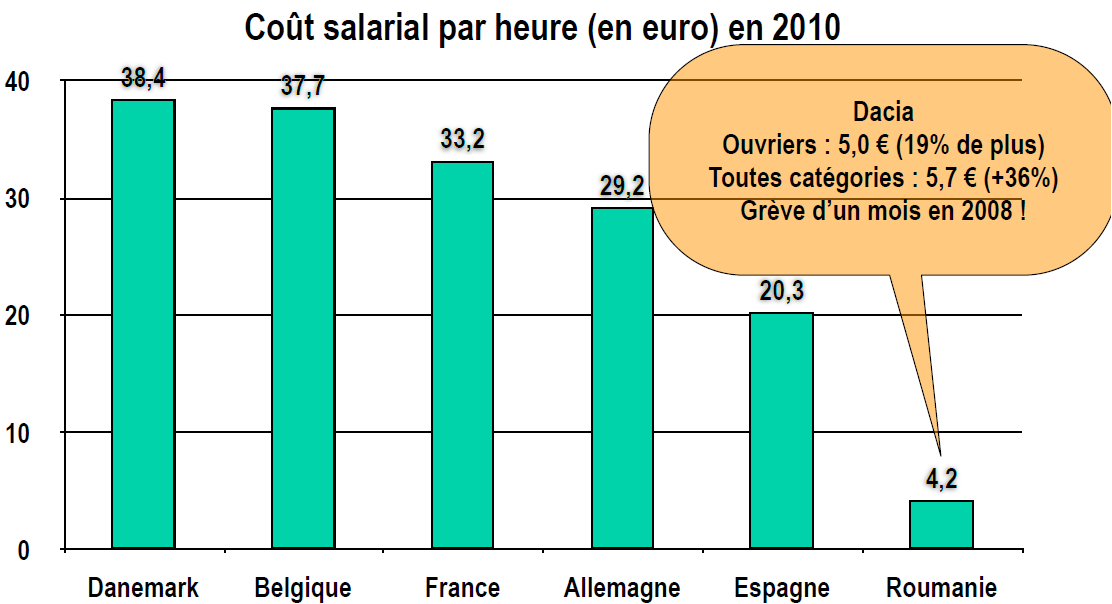
\includegraphics[scale=0.3]{58}
\end{wrapfigure}
Le plus gros avantage de la délocalisation est la présence d'une main d'oeuvre à très bas coûts. On voit que dans les pays développé, le coût est assez haut en raison de toutes les sécurités sociales. Dacia paye quand même 20\% en plus que le coût moyen et avec les contremaître ça monte à 36\%. Ceci est dû au fait que Dacia a du former ses ouvriers au départ. 
\\
On observe quand même que les salaires en Roumanie, Chine et Vietnam augmentent assez vite. On remarque aussi que plus les salaires sont bas plus ils augmentent vite (+16\% de 2010 à 2012 en Roumanie).
\\\\
Dans les fondamentaux de la pensée économique on a \textbf{Adam Smith}, philosophe et économiste écossais. Il est le maître de la pensée classique du libéralisme économique. Il a dit : \textbf{« Il est prudent de ne jamais essayer de faire chez soi la
chose qui coûtera moins à acheter qu’à faire »}. Ca ne sert donc à rien de faire soi même quelque chose, si dans une autre zone géographique on la fait mieux. Faisons ce que nous faisons de meilleurs (meilleur accès aux matières premières, savoir faire, coûts de production plus bas).

\section{Renault au Maroc}
\subsection{Dacia Bis}
Dacia a bien réussi en Roumanie. Renault va cette fois essayer au Maroc aussi. Ils ouvrent une nouvelle usine à Tanger. A l'inverse de la Roumanie là on construit une usine de zéro (greenfield), très grande. Et on produit un nouveau véhicule (Lodgy). Si le marché primaire est le Maroc on veut surtout pouvoir vendre en Europe. \\
Les salaires sont bien plus bas qu'en France, mais on arrive à atteindre 75\% de productivité par rapport à la France. Cette fois on utilise les robots pour avoir une qualité élevée. Cela déclenche des réaction politique très fortes en France !

\subsection{Réactions politiques}
Les politiques, de droite, gauche et d'extrême ont tous le même point de vue. Il ne faut pas que Renault se dirige vers le low cost mais qu'il monte en gamme (Bruno Le Roux) et qu'il produise à l'extérieur des voitures destinées à la France et l'Europe (Christian Estrosi). Louis Aliot (numéro 2 du FN) veut carrément un protectionnisme européen. \\
De l'autre côté, le patron de Renault défend son cas. Il explique que ce n'est pas au détriment de la France. Ca permet de rajouter de l'ingénieurie en France. Les moteurs et la conception sont fait en France. On localise en France les produits les plus sofistiqués. "Si je veux faire du low-cost je ne peux pas le faire en France". De plus, la concurence n'est pas présente puisque Dacia et Renault ont des clients totalement différents. \\
Selon une opinion de syndicat, on se plaint de l'immigration et là c'est l'occasion d'offrir aux étrangers du travail dans leur pays. 

\section{Bénéficiaires et victimes}
Ce sont bien sûr les étrangers qui profitent. Ils ont un meileur revenu et une formation, un déloppement. Les consommateurs Européens aussi en profitent, car le prix est moindre. Les producteurs de matières premières aussi en bénéficient puisque la demande augmente, ainsi que les prix. \\
Par contre, les travailleurs non qualifiés des pays développés sont mal. 

\section{Innovations technologiques}
Tout d'abord, dans quel sens cela fonctionne ? 

\begin{itemize}
	\item Le progrès du bien-être humain est-il la conséquence du progrès technologique et de la croissance économique ? 
	
	\item Le progrès technologique est-il la cause de la croissance économique et la conséquence de la croissance économique ? 
	
	\item Le progrès technologique a-t-il des conséquences négatives sur la croissance économique et sur le bien-être humain ?
\end{itemize}

\subsection{Choix technologiques}
Par definition, les ressources sont rares. On a le travail, les machines, (travail passé rendu efficace), la terre, l'espace disponible et les matières premières. Jusqu'à présent, les gens veulent consommer plus que ce que l'économie peut produire. On va donc choisir ce qu'on va produire. 

\begin{wrapfigure}[9]{l}{8 cm}
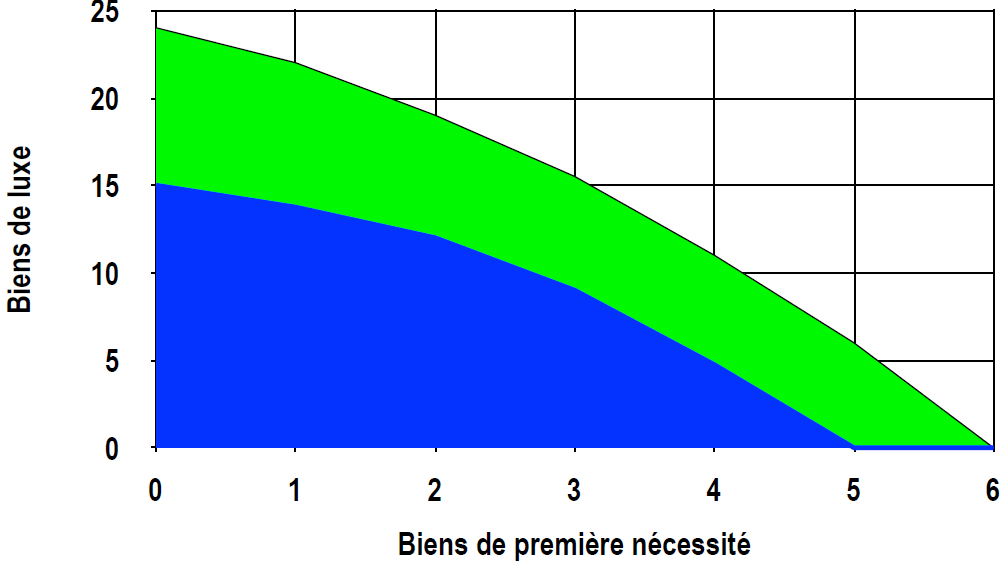
\includegraphics[scale=0.3]{59}
\end{wrapfigure}
L'exemple classique des économiste est la comparaison entre le beurre et le canon. On conceptualise la production de bien de luxe et de première nécéssité. Ce qu'on fait, c'est qu'on va se placer tout le temps en dessous de la courbe max (en bleue) pour ne pas aller à la limie de l'économie. Mais comment aller plus loin en déplaçant cette courbe ? On peut ne rien changer aux technologies en montant la main d'œuvre. Pour cela, on fait amener des travailleurs émigrés. Ou alors, on peut aussi avoir plus de machines, mais pour ça, on va devoir faire des investissements. \\
Le second cas serait en abscence de changement des facteurs de production. Il faudrait alors une meilleure mise en oeuvre de ces facteurs (avancée technologique). On passe dans l'un ou l'autre cas à la courbe verte. 

\section{Innovations}
\subsection{Innovations radicales}
On introduit petit a petit les progrès technologiques. Mais on a parfois des progrès qui entraînent des changements en profondeur des conditions de vie ou de production. On appelle ça les innovations radicales. Avec ces changements, la hausse très forte de la productivité entraîne la baisse de certains prix. On a également de nouveaux biens ou services. Cela fait apparaître donc de nouveaux besoins. En voici quelques exemples : 

\begin{itemize}
	\item La machine à vapeur $\rightarrow$ remplace l’énergie humaine ou animale $\rightarrow$ très forte hausse de productivité et très forte baisse du prix du transport.
	
	\item Le transistor $\rightarrow$ le développement de l’électronique $\rightarrow$ nouveaux produits : télévision, ordinateurs, téléphones portables $\rightarrow$ très forte baisse du coût du traitement de l’information.
	
	\item La péniciline $\rightarrow$ augmentation de l'espérance de vie.
	
	\item Production à la chaîne $\rightarrow$ amélioration importante de la productivité.
	
	\item « Do it yourself » $\rightarrow$ amélioration importante de la productivité du travail rémunéré
\end{itemize}

\subsection{Révolutions industrielles}
\textit{C'est un changement radical du système technico-économique, un ensemble lié d’innovations radicales provoquant un saut de productivité dans la plupart des secteurs
de l’économie.} \\
Les facteurs de déclenchement sont : l'innovation permettant de diminuer vite et fort le prix d'un facteur clé, la disponibilité illimitée des inputs et un large  potentiel d'utilisation. Les deux tableaux ci-dessous reprennent les 5 révolutions industrielles. \\

\begin{minipage}{0.5\textwidth}
	\begin{flushleft}
		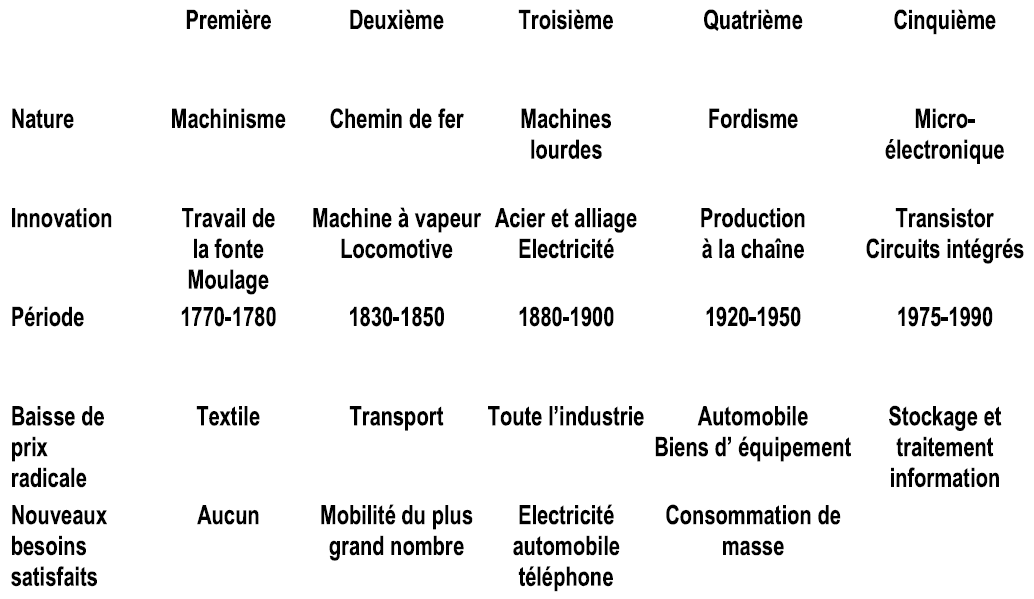
\includegraphics[scale=0.26]{60}
	\end{flushleft}
\end{minipage}
\begin{minipage}{0.5\textwidth}
	\begin{center}
		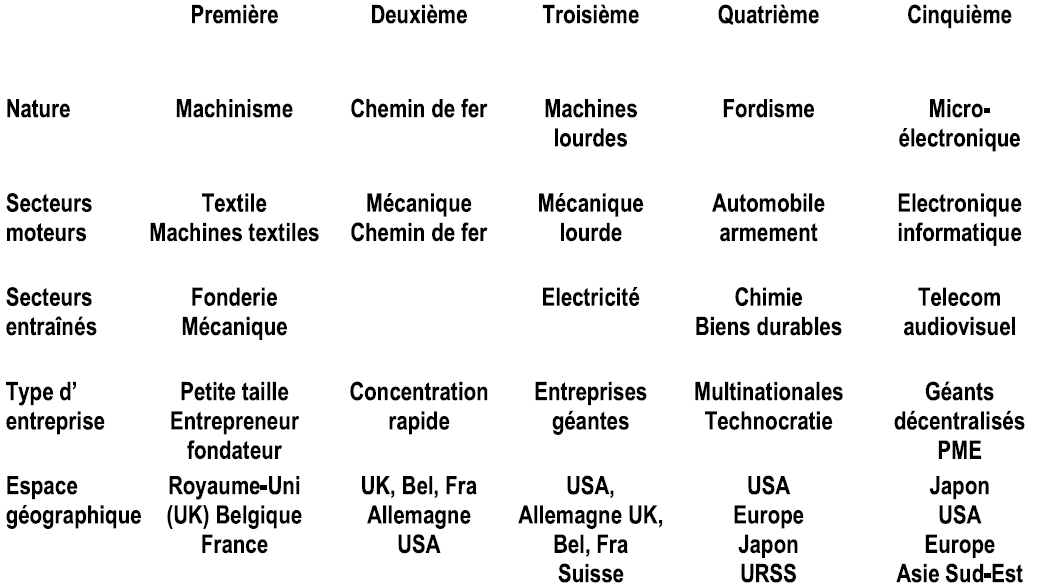
\includegraphics[scale=0.29]{61}
	\end{center}
\end{minipage}
\\\\
Si on regarde les 5 révolutions, elles ont toutes la conditions de la disponibilité illimité du facteur de production (coton, charbon, ...). Il faut également des entrepreneurs innovateurs qui vont porter le progrès loin : 

\begin{itemize}
	\item 3ème révolution : Siemens, Solvay, Marconi, Edison, Eastman
	\item 4ème révolution : Ford
	\item 5ème révolution : Steve Jobs, Bill Gates
\end{itemize}

\section{Facteurs influançant le développement technologique}
\subsection{Condition nécéssaire mais pas suffisante}
\begin{wrapfigure}[11]{l}{10 cm}
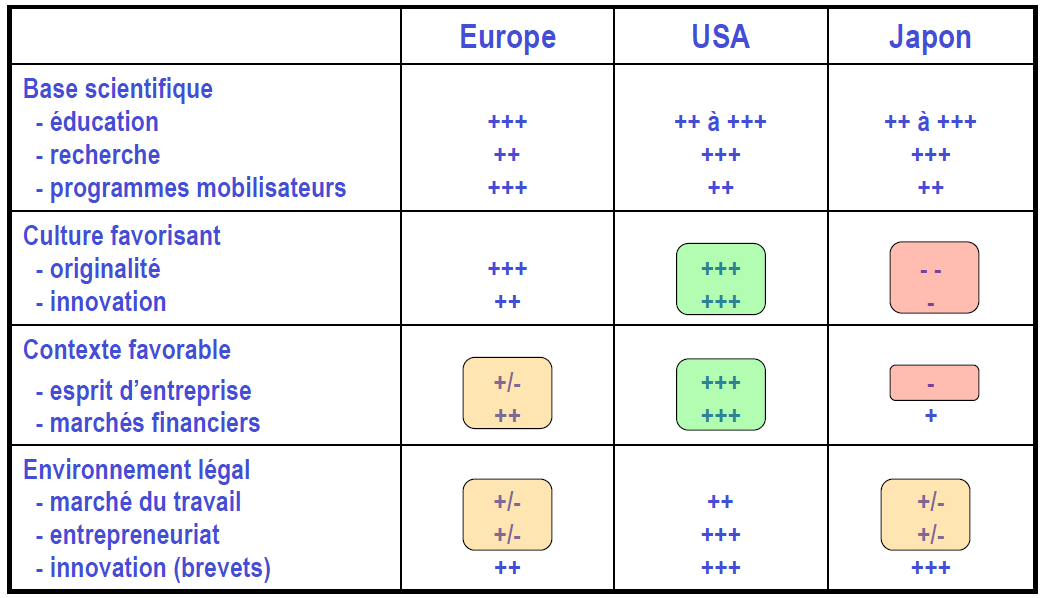
\includegraphics[scale=0.35]{62}
\end{wrapfigure}
Pour stimuler l'innovation, il faut la capacité de former les populations, être capable de développer de la recherche (éducation). La culture doit stimuler la créativité et l'originalité pour permettre les nouveautées. Il faut faire en sorte de traduire le développement en des produits et services concrets (acceptation des risquess et présence des moyens financiers). Finalement, le cadre légal doit stimuler l'innovation et l'entreprise.  

\subsection{Et demain ?}
\begin{wrapfigure}[12]{l}{10 cm}
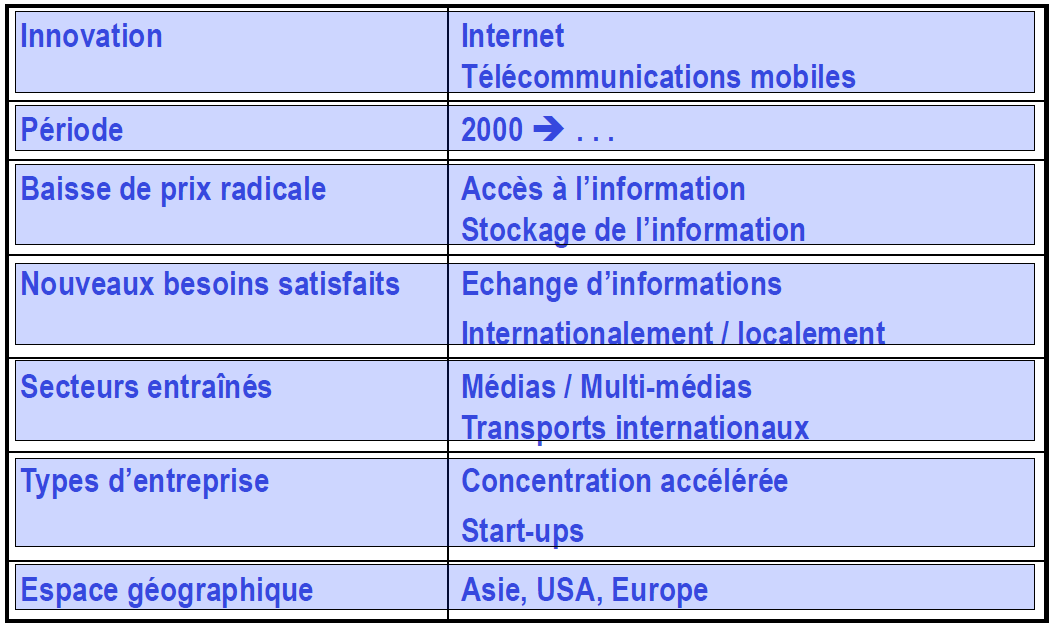
\includegraphics[scale=0.35]{63}
\end{wrapfigure}
Dans la poursuite de ce qu'a rendu possible le transistor, l'innovation se poursuit dans la télécommunication mobile. On a accès très vite à de l'information pour un prix dérisoire. Nouveaux besoins : échange d'informations. Les performances des matériaux continueront à s’améliorer le contenu en énergie va continuer à diminuer et le taux de recyclage va augmenter considérablement. Par ailleurs, le contenu en information va continuer à augmenter. La vitesse de calcul, le volume stockable et transportable augmente, les produits sont adaptés aux besoins, communautés virtuelles, conséquences culturelles (facebook), ... 
\\\\
L’innovation technologique influencera encore plus
l’économie puisque la vitesse de changement et de transmission de l'innovation sera plus grande. Aussi, l'économie influencera encore plus l'innovation puisqu'il y a de plus en plus de concurrence entre les entreprises. 

